\subsection{Neural network used}



\subsection{Use of a BPT to compute the loss}


\subsection{An improved way to generate edge weights}

One of the issues that we had before was that when computing the edge weights we lost the gradient
information, which forced us to go back to our neural network's output, which was costly.
However a change in Higra's function to compute edge weights forced us to adapt and find a better
method, which will describe here.\\

\begin{figure}[!htbp]
	\centering
	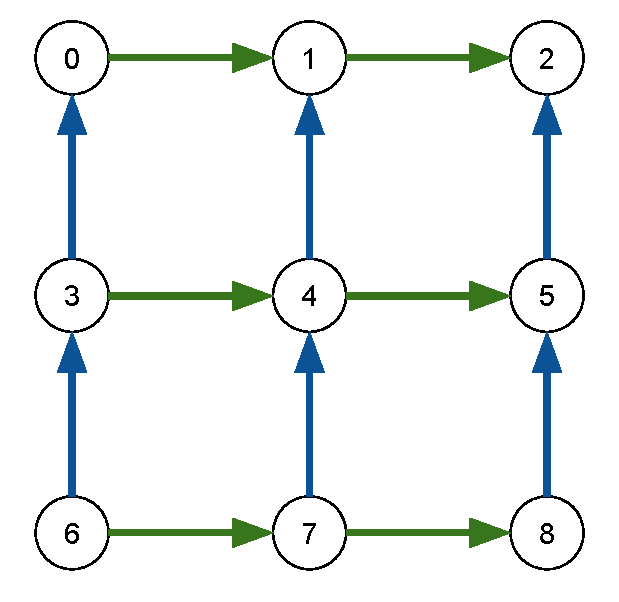
\includegraphics[width=0.5\linewidth]{./images/graph.pdf}
	\caption{Construction of a 4 connected graph in 2d. Green edges represent x
	edges and blue edges represent y edges}%
	\label{fig:graph}
\end{figure}

As we can see in figure~\ref{fig:graph} there is a straightworward way to
relate our edges and their counterpart in the neural network output.\\

The only constraint that we have for the construction of the edge weights is to
use operations supported by our deep learning library of choice. For PyTorch, this
includes if statements, min, max, all array indexing methods etc.

\subsubsection{Weighting edges with Higra}

Once we have our edge weighting function, we can directly use Higra to get our
edge weights.
\begin{lstlisting}[language=Python]
import higra as hg

# Both variables were obtained from our NN
x_edges = ...
y_edges = ...

#Building our graph
graph = hg.get_4_adjacency_graph(x_edges.shape)

#Getting our edges and computing their weights
src, dst = graph.edge_list()
weights = weight_function(src,dst,x_edges,y_edges)
\end{lstlisting}

This will work in the general case, but in the case of a 4 connected graph and
with the way our neural network generates edge weights we can optimise this.
Indeed the edge list is obtained in a structured and deterministic way which
we will now decsribe.

\clearpage
\subsubsection{Higra's edge weights structure}

\begin{figure}[!htbp]
	\centering
	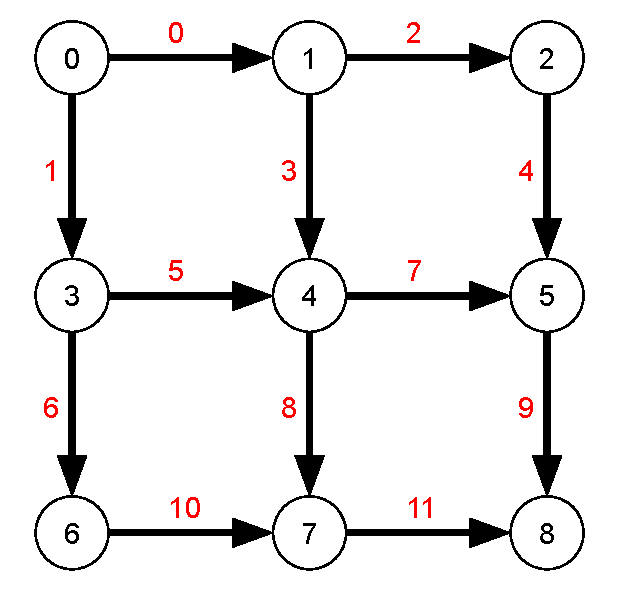
\includegraphics[width=0.5\linewidth]{./images/graph-order.pdf}
	\caption{Oder of edges obtained using Higras's \textit{edge\_list}
	function.}%
	\label{fig:graph_order}
\end{figure}

As we can see in figure~\ref{fig:graph_order} edges are always obtained in the
same fashion, which will allow us to develop a function that bypasses the call
to \textit{edge\_list} since they will always be in the same order.\\
The constraint are thus that we need to respect this order in our function, and
we need to be careful about code maintenance and unit tests, as a change of the
way the edges are obtained would break our method.\\
To alleviate those risks, the best method is to create tests comparing our
method and the official method, which is guaranteed to work.


\subsubsection{Our method to generate edge weights}

\begin{figure}[!htbp]
\centering
\begin{minipage}[c]{0.2\textwidth}
\centering
\[
	\text{x\_edges}=
  \begin{bmatrix}
	  1 & 2 & 3 \\
	  4 & 5 & 6 \\
	  7 & 8 & 9 \\
  \end{bmatrix}
\]
\end{minipage}\hfill
\begin{minipage}[c]{0.2\textwidth}
\centering
\[
	\text{y\_edges}=
  \begin{bmatrix}
	  -1 & -2 & -3 \\
	  -4 & -5 & -6 \\
	  -7 & -8 & -9 \\
  \end{bmatrix}
\]

\end{minipage}\hfill
\begin{minipage}[c]{0.45\textwidth}
\centering
    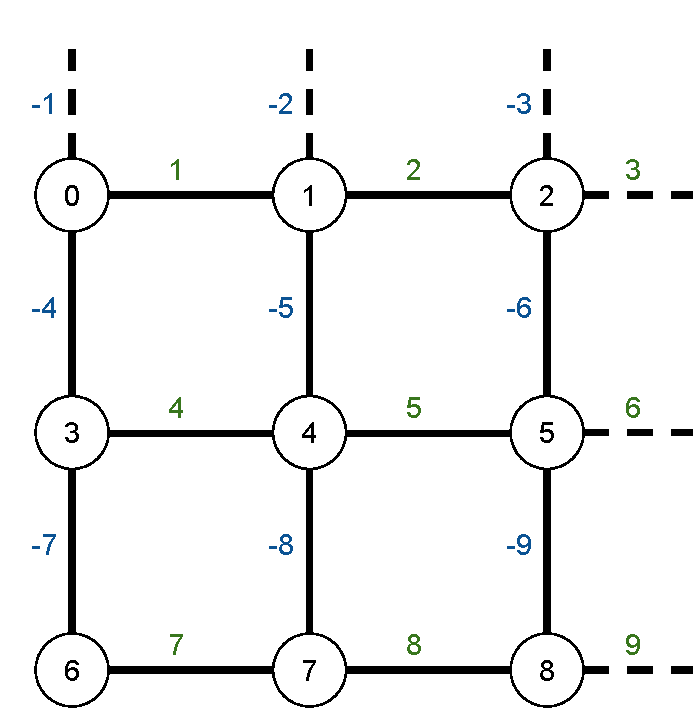
\includegraphics[width=\textwidth]{./images/edge_weights_predicted.pdf}
\end{minipage}

    \caption{Example of desired results from our x and y edges predicted by our
	neural network. Notice that some edges are not contained in the image. Even
though they are present in our NN output we will remove them from the graph}
    \label{fig:ew_predicted}
\end{figure}

As we can see in figure~\ref{fig:ew_predicted}, we get edge matrices the same
size as our image, but if our image is of dimension $n\times m$ we only need a
matrix of size $n\times (m-1)$ for our edges in the y direction and of size
$(n-1)\times m$ for our edge in the x direction.\\
The choice to have those irrelevant edge weights is simply for ease of use, and
to ease the design of the NN output.\\

As we can also see, our edge weights are simply a
kind of entanglement of our x and y edges. This leads us to the following code
to generate of edge weights which doesn't rely on Higra's function :
\begin{lstlisting}[language=Python]
import higra as hg
import torch

# Both variables were obtained from our NN
x_edges = ...
y_edges = ...

# Getting our edge weights

height,width=x.shape
# Removing the out of graph edges
x_u  = x_edges[:-1].T[:-1]
y_u = y_edges[1:].T

edge_weights = torch.from_numpy(np.empty((2*width-1,height-1),dtype=np.float64))
edge_weights = edge_weights.type(torch.FloatTensor).to(device)

# Creating the entanglement
edge_weights[0:-1:2,:] = x_u
edge_weights[1::2,:] = y_u[:-1]
edge_weights[-1] = y_u[-1]

#Adding back missing x edges
edge_weights= torch.cat((edge_weights.T.flatten(),x_edges[-1,:-1]))
\end{lstlisting}

This example here is using PyTorch, but an analogous version for numpy can be
made by replacing function names.\\

Using this code we are able to generate edge weights very fast and we are sure
that our edge weights will contain the gradient history, which is what we
wanted.

\subsubsection{Backpropagation}

Once we have our edge weights as an array, for any processing that we will have
to do, we can refer to the edge weights which are guaranteed to contain the
gradient information. This is easier that going back to the NN output, where we
would have to reverse the code used to get our edge weights to find their
position in the output.\\

This process of going back to our neural network was very costly and caused a
very important bottleneck in our code, which this solution alleviated
instantly. We had a backward pass that was taking 100 times as long as our
forward pass, which should not be the case, we expected it to be 2 or 3 times
as ong at most.
